% -*- mode: LaTeX; TeX-PDF-mode: t; -*- # Tell emacs file type (for syntax coloring)
% LaTeX path to the root directory of the current project, from the directory in which this file resides
% and path to econtexPaths which defines the rest of the paths like \FigDir
\providecommand{\econtexRoot}{}\renewcommand{\econtexRoot}{.}

\documentclass[\econtexRoot/Letter]{subfiles}
\onlyinsubfile{\externaldocument{\econtexRoot/Letter}} % Get xrefs -- esp to apndx -- from main file; only works if main file has already been compiled

\begin{document}
\notinsubfile{\renewcommand{\econtexRoot}{.}}

\hypertarget{job-market-paper}{}
%\par\section{Job Market Paper}
\notinsubfile{\label{sec:job-market-paper}}

%[Description of JMP and any other relevant work] \\

Will's job market paper is my favorite kind of exercise: Take some well-established microeconomic fact, incorporate it into a HA macro model, and show that it has interesting macro implications that are not present until you match the micro reality. In Will's case, the micro fact is that exogenous spells of unemployment have a ``scarring effect'' on subsequent earnings. The micro literature has made the usual heroic efforts to establish that the measured scars are not due to some form of selection on unobservables - they are, as best one can tell, a causal consequence of an exogenous unemployment shock.  The simplest interpretation is that the spell results in a negative shock to idiosyncratic human capital.  (Other explanations, like a job ladder or match quality, would have the same consequences).  Such shocks are therefore far more consequential than the kinds of unemployment spells incorporated pervasively in standard HA (especially HANK) models.  Will modifies a standard HANK model so that the micro unemployment process can match the scarring facts, and explores the consequences in a particular dimension: The consequences of a recession for subsequent output.  Consistent with the old literature suggesting that there is a unit root in GDP, Will finds that in his HANK model a recession results in a permanent reduction in the level of GDP because the shocks to human capital are permanent. These results connect not only with the old unit root and ``hysteresis'' literatures, but also with the newer ``secular stagnation'' literature.  To gauge the magnitude of the effects, Will does an exercise to compare the aftermath of the Great Recession in the United States and in the Euro zone, motivated by the fact that in Europe the byword for the fiscal response to the GR was ``austerity'' while in the US there was considerable stimulus (and a litany of criticism that the US should be pursuing austerity not stimulus). In Will's model, as in the data, the stimulative policy results in a much lower permanent drop in GDP than the austerity policy, corresponding to the actual outcomes in the US versus Europe.

% Put here a link to the abstract of the JMP:

%%% Template for any figures
%\begin{figure}[ht!]
%	\centering
%	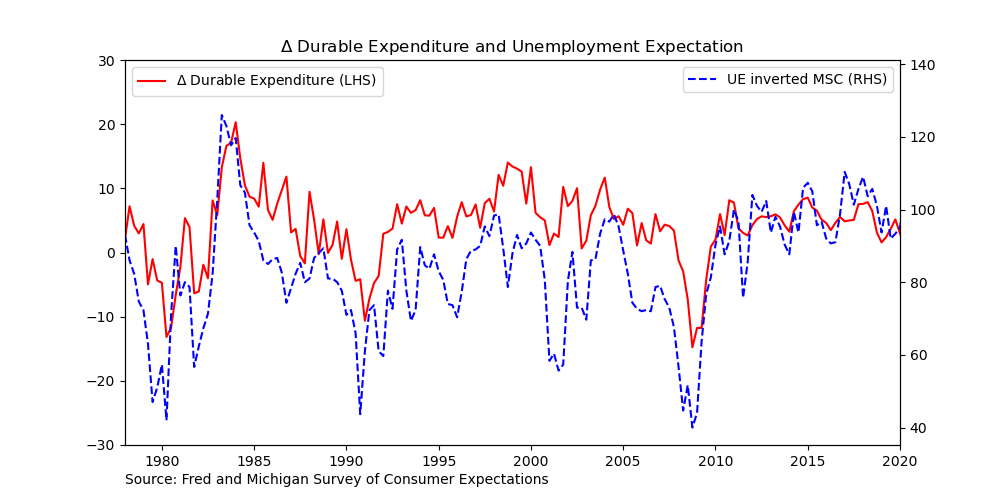
\includegraphics[width = 0.8\textwidth]{\FigDir/dur_vs_exp_emp.png}
	%\caption{Durable Expenditure and Expected Unemployment Rate} \label{fig:dur_vs_exp_emp}
%\end{figure}

\onlyinsubfile{% Allows two (optional) supplements to hard-wired \texname.bib bibfile:
% system.bib is a default bibfile that supplies anything missing elsewhere
% Add-Refs.bib is an override bibfile that supplants anything in \texfile.bib or system.bib
\provideboolean{AddRefsExists}
\provideboolean{systemExists}
\provideboolean{BothExist}
\provideboolean{NeitherExists}
\setboolean{BothExist}{true}
\setboolean{NeitherExists}{true}

\IfFileExists{\econtexRoot/Add-Refs.bib}{
  % then
  \typeout{References in Add-Refs.bib will take precedence over those elsewhere}
  \setboolean{AddRefsExists}{true}
  \setboolean{NeitherExists}{false} % Default is true
}{
  % else
  \setboolean{AddRefsExists}{false} % No added refs exist so defaults will be used
  \setboolean{BothExist}{false}     % Default is that Add-Refs and system.bib both exist
}

% Deal with case where system.bib is found by kpsewhich
\IfFileExists{/usr/local/texlive/texmf-local/bibtex/bib/system.bib}{
  % then
  \typeout{References in system.bib will be used for items not found elsewhere}
  \setboolean{systemExists}{true}
  \setboolean{NeitherExists}{false}
}{
  % else
  \typeout{Found no system database file}
  \setboolean{systemExists}{false}
  \setboolean{BothExist}{false}
}

\ifthenelse{\boolean{showPageHead}}{ %then
  \clearpairofpagestyles % No header for references pages
  }{} % No head has been set to clear

\ifthenelse{\boolean{BothExist}}{
  % then use both
  \typeout{bibliography{\econtexRoot/Add-Refs,\econtexRoot/\texname,system}}
  \bibliography{\econtexRoot/Add-Refs,\econtexRoot/\texname,system}
  % else both do not exist
}{ % maybe neither does?
  \ifthenelse{\boolean{NeitherExists}}{
    \typeout{bibliography{\texname}}
    \bibliography{\texname}}{
    % no -- at least one exists
    \ifthenelse{\boolean{AddRefsExists}}{
      \typeout{bibliography{\econtexRoot/Add-Refs,\econtexRoot/\texname}}
      \bibliography{\econtexRoot/Add-Refs,\econtexRoot/\texname}}{
      \typeout{bibliography{\econtexRoot/\texname,system}}
      \bibliography{        \econtexRoot/\texname,system}}
  } % end of picking the one that exists
} % end of testing whether neither exists
}

\ifthenelse{\boolean{Web}}{}{
  \onlyinsubfile{\captionsetup[figure]{list=no}}
  \onlyinsubfile{\captionsetup[table]{list=no}}
  \end{document}	\endinput
}

